% !Mode:: "TeX:UTF-8" 



\BiSection{2.21}{Figures}

\fancyhead[R]{本题2.21由QC.Z完成}



解:

连接欧姆表的MOSFET简单图如图1所示

		\begin{figure}[H] %H为当前位置,!htb为忽略美学标准,htbp为浮动图形
	\begin{minipage}{\linewidth}
		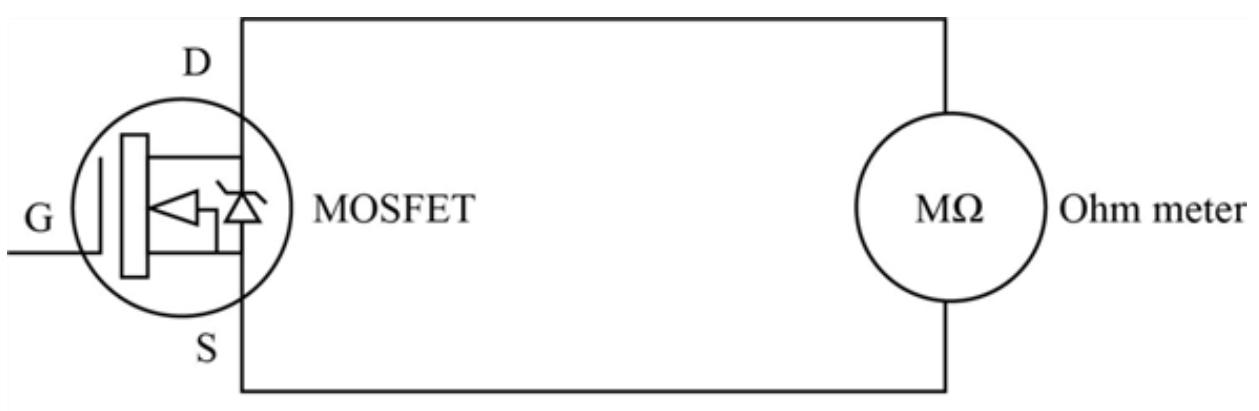
\includegraphics[width=1\linewidth]{2.21-1}
	\end{minipage}
	\caption*{图1} %最终文档中希望显示的图片标题
\end{figure}


先找衬底源和衬底漏。欧姆表每次连2个引脚,12种测量中只有2次低阻(因为pn结外加正偏电压产生电流)

最后判断低阻时正表头连接的是衬底,负表头连源/漏,剩下的引脚是栅

















%每次用欧姆表测2个引脚,最多测6次;其中只有2次低阻(因为pn结外加正偏电压产生电流),其余测量呈现高阻;低阻时正表头连接的是衬底,负表头连源/漏,剩下的引脚是栅;最少测2次


















%每次用欧姆表测正表头连1个引脚、负表头连1个引脚;正表头不动,负表头测完3个引脚再动正表头;最多用9次测量找衬底源和衬底漏\textcolor{blue}{(最糟糕情况下先测出栅和源/漏,最后3次不用测量。3次负表头高阻则正表头为栅,2次负表头高阻则正表头为衬底,1次负表头高阻则正表头为源/漏)}
%
%正表头不动的每3次测量中,若只有2次测量低阻(因为pn结外加正偏电压产生电流),其余测量呈现高阻,则找到衬底源和衬底漏;低阻时正表头连接的是衬底,负表头连源/漏,剩下的引脚是栅,最少测量3次







%把欧姆表的负表头连MOSFET的衬底,另一个表头分别连剩下两端,高阻则为地,低阻则为源/漏
%
%因为衬底的帮助,最坏的情况下需要8次测量







